\chapter{Theory}
\label{cha:theory}

% The main purpose of this chapter is to make it obvious for
% the reader that the report authors have made an effort to read
% up on related research and other information of relevance for
% the research questions. It is a question of trust. Can I as a
% reader rely on what the authors are saying? If it is obvious
% that the authors know the topic area well and clearly present
% their lessons learned, it raises the perceived quality of the
% entire report.
% 
% After having read the theory chapter it shall be obvious for
% the reader that the research questions are both well
% formulated and relevant.
% 
% The chapter must contain theory of use for the intended
% study, both in terms of technique and method. If a final thesis
% project is about the development of a new search engine for
% a certain application domain, the theory must bring up related
% work on search algorithms and related techniques, but also
% methods for evaluating search engines, including
% performance measures such as precision, accuracy and
% recall.
% 
% The chapter shall be structured thematically, not per author.
% A good approach to making a review of scientific literature
% is to use \emph{Google Scholar} (which also has the useful function
% \emph{Cite}). By iterating between searching for articles and reading
% abstracts to find new terms to guide further searches, it is
% fairly straight forward to locate good and relevant
% information, such as \cite{test}.
% 
% Having found a relevant article one can use the function for
% viewing other articles that have cited this particular article,
% and also go through the article’s own reference list. Among
% these articles on can often find other interesting articles and
% thus proceed further.
% 
% It can also be a good idea to consider which sources seem
% most relevant for the problem area at hand. Are there any
% special conference or journal that often occurs one can search
% in more detail in lists of published articles from these venues
% in particular. One can also search for the web sites of
% important authors and investigate what they have published
% in general.
% 
% This chapter is called either \emph{Theory, Related Work}, or
% \emph{Related Research}. Check with your supervisor.

This chapter introduces relevant theory and related work.
Section ~\ref{sec:activevision} gives some background on active vision.
Section ~\ref{sec:visualsearch} describes the problem of visual searching for targets.

% describe how animal vision translates to camera vision?
% animals have a large field of view, but also require foveated vision: processing is expensive.
% computers do not naturally have this constraint and most CV algorithms do not use foveated vision
% (although visual attention models exist)

\section{Search in Partially Observable Environments}
% Artificial Intelligence - A modern approach
% Should cover belief states?

\section{Active Vision}
\label{sec:activevision}

% Marr?

Much of past and present research in machine perception involves a passive observer.
Images are passively sampled and perceived.
Animal perception, however, is active.
We do not only see things, but look for them.
One might ask why this is the case, if there is any advantage that an active observer has over a passive one.
Aloimonos and Weiss (1988)~\cite{aloimonos_active_1988} introduce the paradigm called \textit{active vision}, and prove that an active observer can solve several basic vision problems in a more efficient way than a passive one.

Bajcsy (1988)~\cite{bajcsy_1988} defines active vision, and perception in general, as a problem of intelligent data acquisition.
An active observer needs to define and measure parameters and errors from its scene and feed then back to control the data acquisition process.
Bajscy states that one of the difficulties of this problem is that they are scene and context dependent.
A thorough understanding of the data acquisition parameters and the goal of the visual processing is needed.
One view lacks information that may be present with multiple views.
Multiple views also add the time dimension into the problem.

In a re-visitation of active perception, Bajcsy, Aloimonos and Tsotsos (2018)~\cite{bajcsy_aloimonos_tsotsos_2018} stress that despite recent successes in robotics, artificial intelligence and computer vision, an intelligent agent must include active perception:

\begin{quote}
    An agent is an active perceiver if it knows why it wishes to sense, and then chooses what to perceive, and determines how, when and where to achieve that perception
\end{quote}~\cite{bajcsy_aloimonos_tsotsos_2018}

% see conclusion in that paper:
% - mirror neurons, same system responsible for generating and interpreting actions at a high level 

\section{Visual Search}
\label{sec:visualsearch}

The perceptual task of searching for something in a visual environment is usually referred to as \textit{visual search}.
The searched object or feature is the \textit{target}, and the other objects or features in the environment are the \textit{distractors}.
This task has been studied extensively in psychology and neuroscience.

Wolfe (2021)~\cite{wolfe_guided_2021} describes a model of visual search

% general things
% - foveated vision
% - covert and overt attention
% ...

Eckstein (2011)~\cite{eckstein_visual_2011} reviews efforts from various subfields and identifies a set of mechanisms used to achieve efficient visual search.
Knowledge about the target, distractor, background statistical properties, location probabilities, contextual cues, rewards and target prevalence are all identified as useful.
This is motivated with evidence from psychology as well as neural correlates.

Visual search is not always instant, and can in fact often be slow.
This is in part due to processing: our visual system cannot process the entire visual field and 

% saliency, center-surround organization
% covert attention and eye movement

Wolfe and Horowitz (2017)~\cite{wolfe_horowitz_2017} identify and measure a set of factors that guide attention in visual search.
One of these is bottom-up guidance, in which some visual properties of the scene draw more attention than others.
Another is top-down guidance, which is user driven and directed to objects with known features of desired targets.
Scene guidance is also identified, in which attributes of the scene guide attention to areas likely to contain targets. 

These works ground the task considered in this project in psychology.

% can we build a system that exhibits all of these?

\section{Object Detection}

% active object detection

A similar problem can be found in the computer vision literature under \textit{object detection}.
The goal of object detection is to, given an input image, detect instances of semantic objects in it.
This includes assigning a bounding box to the objects, and classifying the object.
The input image is usually passively sampled, and the whole scene is visible at once.

Caicedo and Lazebnik (2015)~\cite{aol} propose to use deep reinforcement learning for active object localization in images where the object to be localized is fully visible.
An agent is trained to successively improve a bounding box using translating and scaling transformations.
They use a reward signal that is proportional to how well the current box covers the target object.
An action that improves the region is rewarded with +1, and -1 otherwise.
Without this quantization, the difference was small enough to confuse the agent.
Binary rewards communicate more clearly which transformations keep the object inside the box and which take the box away from the target.
When there is no action that improves the bounding box, the agent may select a trigger action (which would be the only action that does not give a negative reward) which resets the box.
This way the agent may select additional bounding boxes.
Each trigger modifies the environment by marking it so that the agent may learn to not select the same region twice.
This is referred to as an inhibition-of-return mechanism, and is widely used in visual attention models~\cite{16 in aol}.
This method has a few shortcomings for the problem considered in this project.
The object may not be visible in the initial frame so the agent cannot act in the same way. 

A separate field is active object search, which is perhaps most closely related to the problem we consider in this work.
In active object search, % explain
% difference is tht this is the first deep dive into these particular aspects
% write about the work that uses object co-occurences though
% we should stress that we do not explicitly model the environment guidance, but are rather interested in whether it can be learned efficiently by the system

\section{Visual Attention}

% this article is very good!
% note: reinforcement learning part, soft and hard attention
% https://shairozsohail.medium.com/a-survey-of-visual-attention-mechanisms-in-deep-learning-1043eb25f343

\section{Neural Networks}

An artificial neural network (ANN) is a type of universal function approximator

\subsection{Multi-layer Perceptron}

\subsection{Long Short-Term Memory}

\subsection{Convolutional Neural Network}

\section{Reinforcement Learning}

Reinforcement learning (RL) is a subfield of machine learning concerned with learning from interaction how to achieve a goal.
An \textit{agent} and its \textit{environment} interact continually over discrete time steps.
At each time step the agent selects some \textit{action} that updates the state of the environment, and gives it a \textit{reward}.
The agent selects actions using a stochastic \textit{policy} with the goal of maximizing the \textit{return} which is usually defined as the discounted sum of future rewards.~\cite{sutton_reinforcement_2018}

\subsection{Markov Decision Process}

% should likely be its own separate section
% take inspiration from other works?

The RL setup is usually formalized as a (finite) Markov decision process (MDP).

The problem of learning from interaction to achieve a goal is usually framed as a (finite) Markov Decision Process (MDP).
For regular MDPs it is assumed that the learning agent has access to some representation of the underlying \textit{state} of the environment which it uses to select \textit{actions}.
For many problems this is not true.
A partially observable Markov decision process (POMDP) is a generalization of an MDP in which it is assumed that the environment has some well defined underlying latent state, but the agent only perceives a partial \textit{observation} of it from the environment. 

A POMDP is formally defined as a 7-tuple \(\langle \mathcal{S}, \mathcal{A}, \mathcal{O}, \mathcal{R}, \mathcal{T}, \Omega, \gamma \rangle\), where

\begin{itemize}
    \item \(\mathcal{S}\) is a finite set of states,
    \item \(\mathcal{A}\) is a finite set of actions,
    \item \(\mathcal{T}\) is a set of conditional state transition probabilities,
    \item \(\mathcal{R} : S \times A \rightarrow \mathbb{R}\) is a reward function,
    \item \(\Omega\) is a finite set of observations,
    \item \(\mathcal{O}\) is a set of conditional observation probabilities, and
    \item \(\gamma \in [0, 1]\) is a discount factor.
\end{itemize}

\begin{figure}
    \centering
    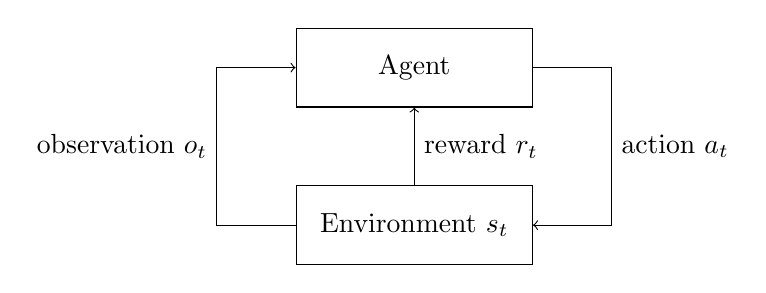
\begin{tikzpicture}[node distance=2cm]
    \tikzstyle{block} = [rectangle,minimum width=3cm,minimum height=1cm,text centered,draw=black,fill=white]
    \node (agent)[block]{Agent};
    \node (environment)[block,below of=agent]{Environment \(s_t\)};
    \draw [->] (agent.east) -- ++(1cm,0) -- node [anchor=west]{action \(a_t\)} ++(0,-2cm) -- (environment.east);
    \draw [->] (environment.north) -- node [anchor=west]{reward \(r_t\)} (agent.south);
    \draw [->] (environment.west) -- ++(-1cm,0) -- node [anchor=east]{observation \(o_t\)} ++(0,+2cm) -- (agent.west);
\end{tikzpicture}
    \label{fig:pomdp}
    \caption{Partially observable Markov decision process.}
\end{figure}

The agent interacts with the environment at discrete time steps \(t = 0, 1, 2, \dots T\). At each time step \(t\), the agent receives an observation of the environment's state \(O_t \in \Omega\) and selects some action \(A_t \in \mathcal{A}\).
In the next time step the agent receives a reward

action \(a \in \mathcal{A}\) which causes the environment to transition to state \(s^\prime\) with probability \(\mathcal{T}(s^\prime | s, a)\).
It receives an observation \(o \in \Omega\) with probability \(\mathcal{O}(o | s^\prime, a)\), as well as a reward \(r\) given by \(\mathcal{R}(s, a)\).

This interaction is repeated until the end of the episode at time step \(T\).
The goal of the agent is to maximize the \textit{discounted return}, defined as the discounted sum of future rewards \(G_t \doteq \sum_{k=t+1}^T \gamma^{k-t-1} R_{k}\) where \(\gamma\) reflects the uncertainty of the environment.

%An MDP satisfies the Markov property: the process is memoryless. A POMDP is not memoryless, as observations only convey part of the underlying state. However, the \textit{history} \(H_t = A_0, O_1, R_1, \dots, A_{t-1}, O_t, R_t\) does.

Planning in a POMDP is undecidable, and solving them is often computationally intractable.
Approximate solutions are more common.

% Belief state

\subsection{Policies and Value Functions}

Most RL algorithms estimate both a \textit{value function} that tells the agent how good it is to be in a given state, and a 

% Deep Reinforcement Learning

\subsection{Policy Optimization}

This work will focus on policy optimization algorithms.

\subsection{Actor Critic Models}

\subsection{Exploration and Exploitation}

% The thesis could also be called Efficient Exploration

% Go into motivation if we use this

% Custom rewards are often needed
% intrinsic?

\subsection{Generalization}

% reality is dynamic
% agents need to be robust to variation
% capability to transfer and adapt to unseen but similar environments
% most current research works on benchmarks that do not test this (MuJoCo, Arcade learning environment)

% refer to survey
% specifically IID (train_dist = test_dist) and OOD environments (train_dist != test_dist)

% how do they handle training and test set?

Kobbe et al. (2020)~\cite{} study generalization in RL. They introduce a benchmark of procedurally generated i.i.d. environments, and find that this is essential to 

\section{Automating Visual Search}

% CT scan material: there is way less variance, otherwise similar. Big difference is that we look at more variance in many aspects?

% CV material: different in that the object is assumed to be visible
